\subsection{ARC-Challenge (Advanced Reasoning Challenge)}
{{\footnotesize
\noindent The AI2 Reasoning Challenge (ARC) Challenge set comprises 7,787 natural, grade-school
science questions that retrieval-based and word co-occurrence algorithms both fail, 
requiring advanced reasoning over a 14-million-sentence corpus.


\begin{description}[labelwidth=4cm, labelsep=1em, leftmargin=4cm, itemsep=0.1em, parsep=0em]
  \item[date:] 2018-03-14
  \item[version:] 1
  \item[last\_updated:] 2018-03-14
  \item[expired:] false
  \item[valid:] yes
  \item[valid\_date:] 2018-03-14
  \item[url:] \href{https://allenai.org/data/arc}{https://allenai.org/data/arc}
  \item[doi:] 10.48550/arXiv.1803.05457
  \item[domain:]
    - Computational Science \& AI
  \item[focus:] Grade-school science with reasoning emphasis
  \item[keywords:]
    - grade-school
    - science QA
    - challenge set
    - reasoning
  \item[licensing:] Apache 2.0 License
  \item[task\_types:]
    - Multiple choice
  \item[ai\_capability\_measured:]
    - Commonsense and scientific reasoning
  \item[metrics:]
    - Accuracy
  \item[models:]
    - GPT-4
    - Claude
  \item[ml\_motif:]
    - Reasoning \& Generalization
  \item[type:] Benchmark
  \item[ml\_task:]
    - Supervised Learning
  \item[solutions:] 0
  \item[notes:] Good
  \item[contact.name:] unknown
  \item[contact.email:] unknown
  \item[datasets.links.name:] Hugging Face
  \item[datasets.links.url:] \href{https://huggingface.co/datasets/allenai/ai2\_arc}{https://huggingface.co/datasets/allenai/ai2\_arc}
  \item[results.links.name:] ARC-Solvers
  \item[results.links.url:] \href{https://github.com/allenai/arc-solvers}{https://github.com/allenai/arc-solvers}
  \item[fair.reproducible:] Yes
  \item[fair.benchmark\_ready:] Yes
  \item[id:] arc-challenge\_advanced\_reasoning\_challenge
  \item[Citations:] \cite{allenai:arc}
\end{description}

{\bf Ratings:} ~ \\

\begin{tabular}{p{0.15\textwidth} p{0.07\textwidth} p{0.7\textwidth}}
\hline
Rating & Value & Reason \\
\hline
dataset & 5 & Data accessible, offers instructions on how to download the data via CLI tools. Splits provided on Huggingface
 \\
documentation & 5 & Explains all necessary information inside a paper
 \\
metrics & 5 & All questions in the dataset are multiple choice, all have a correct answer
 \\
reference\_solution & 5 & Reference solution is available and containerized
 \\
software & 5 & Code is available and well documented for evaluation.
 \\
specification & 4 & Task is clear and inputs/outputs are provided along with format on dataset card.
 \\
\hline
\end{tabular}

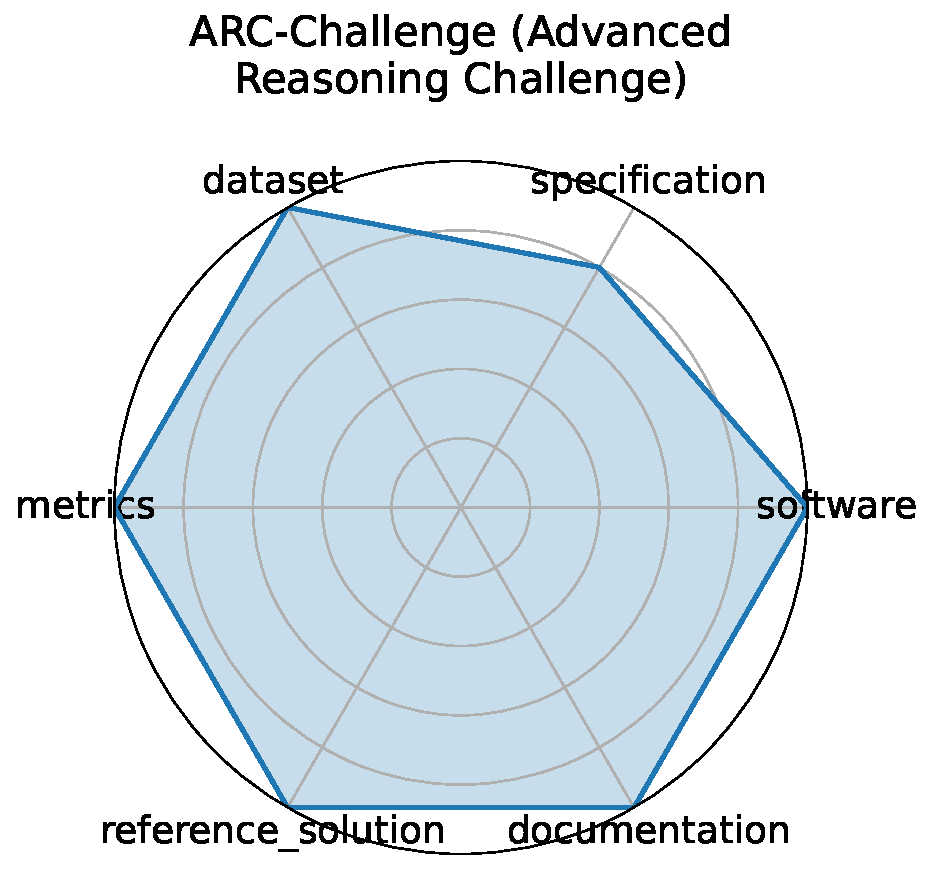
\includegraphics[width=0.2\textwidth]{arc-challenge_advanced_reasoning_challenge_radar.pdf}
}}
\clearpage